%!TEX root = spadini_davide.tex

\chapter{Evaluation}
\label{cha:evaluation}
We now want to evaluate our implementation of the WPSS algorithm, and compare what we obtain with the original papers~\cite{wormhole} in order to confirm or contest their results. We tested our implementation both in deployment and in simulation, however due to the low number of nodes in the real environment we report only the results obtained in simulation. We want to show that our implementation provides the desirable PSS properties, such as fresh samples, randomness, and low cost in a real environment, but also we want to test robustness under different level of churn.

The structure is shown in Fig.~\ref{fig:overlay}, the base overlay is a random undirected graph that is also NAT-friendly, where private nodes are connected to public nodes, and public nodes are connected to one another. The bootstrap service component provides addresses of random public nodes that are used to build the base overlay and to create wormholes. It is implemented as a central server, the tracker. The base overlay service strives to keep the overlay connected repairing broken links, thus, maintaining a fixed number of outgoing links at each node. Every node maintains 20 links to random public nodes, however these links are bidirectional, so the effective average degree is 40. 

We set $TTL = 100$. As discussed in~\cite{wormhole} and also as we will see later, WPSS messages will always terminate much sooner in most practical settings, so the TTL is not a critical parameter.

\section{Experimental Setup}
\label{sec:exp_setup}
For what concerns simulations, we implemented WPSS using the \textbf{Hivejs-Framework-Sim} provided by the Hive Streaming company. It is very configurable, and it allows us to define the network size, the bandwidth of the nodes but also to test the implementation under different level of churn or latency. All experiments are averaged over 4 runs. We applied the same settings as in the original paper, which are: 

\begin{itemize}
	\item the view size (the number of freshest random samples a node remembers) is set to 50
	\item we set $\Delta = 1$ second
	\item we use a scenario of $N = 1000$ nodes that join following a Poisson distribution with a mean inter-arrival time of 100 milliseconds
\end{itemize}

In all simulations 20\% of the nodes is public and 80\% is private, which, according to~\cite{wormhole}, reflects the distribution observed in the commercial deployments of their P2P application.

\section{Freshness}
\label{sec:eval_freshness}
In this experiment we want to measure the freshness of the samples using the average hop count but also the \textit{$90^{th}$} and \textit{$99^{th}$} percentiles. This is the same test reported in~\cite{wormhole}. Fig.~\ref{fig:my_average_hop_count} shows our result, while in Fig.~\ref{fig:paper_average_hop_count} shows their test. As we can see the result is almost identical, this means that our implementation does not alter this property. In the figure we can notice that the average hop count and the $90^{th}$ percentile grow slowly with increasing of $\Delta_{wh}$, which is the wormhole renewal timer, while the $99^{th}$ percentile grows more quickly. This was expected, since the higher the timer, the more nodes the advertisement will need to traverse in order to find a node which does not already have its sample. An important fact to notice is that the \textit{TTL} is never reached, actually in the worst case it is not greater then 20. Another important result here is that the performance is optimal for $\Delta_{wh}$  between about 5 and 10 seconds, as in their result. Given this finding, we set $\Delta_{wh} = 10$ for the remaining experiments, as this value has good freshness (even considering the $99^{th}$ percentile), while the number of new links required is relatively low (a new connection every $10$ rounds of the algorithm). 

\begin{figure}[ht]
  \centering
  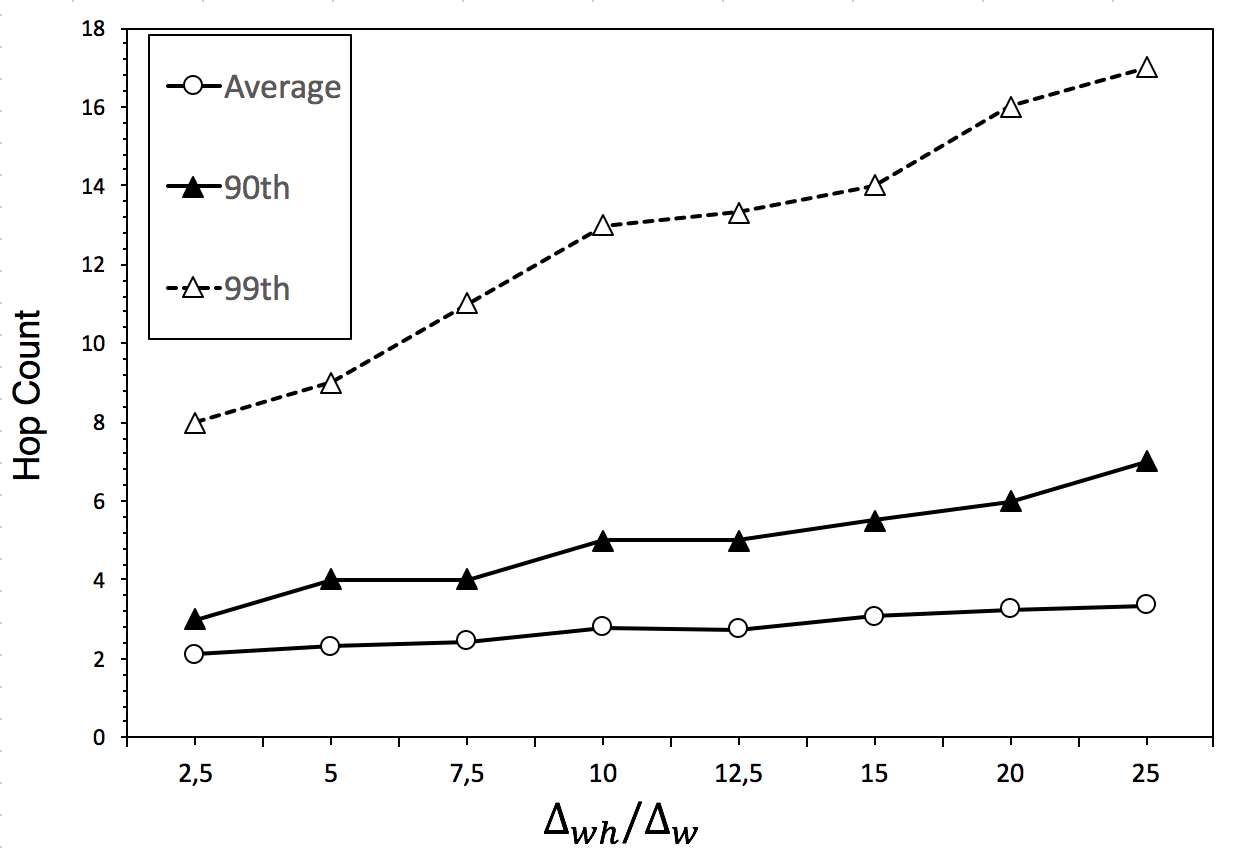
\includegraphics[keepaspectratio=true, width=\textwidth]{images/average_hop_count}\caption{Average hop count}
  \label{fig:my_average_hop_count}
\end{figure}

\begin{figure}[ht]
  \centering
  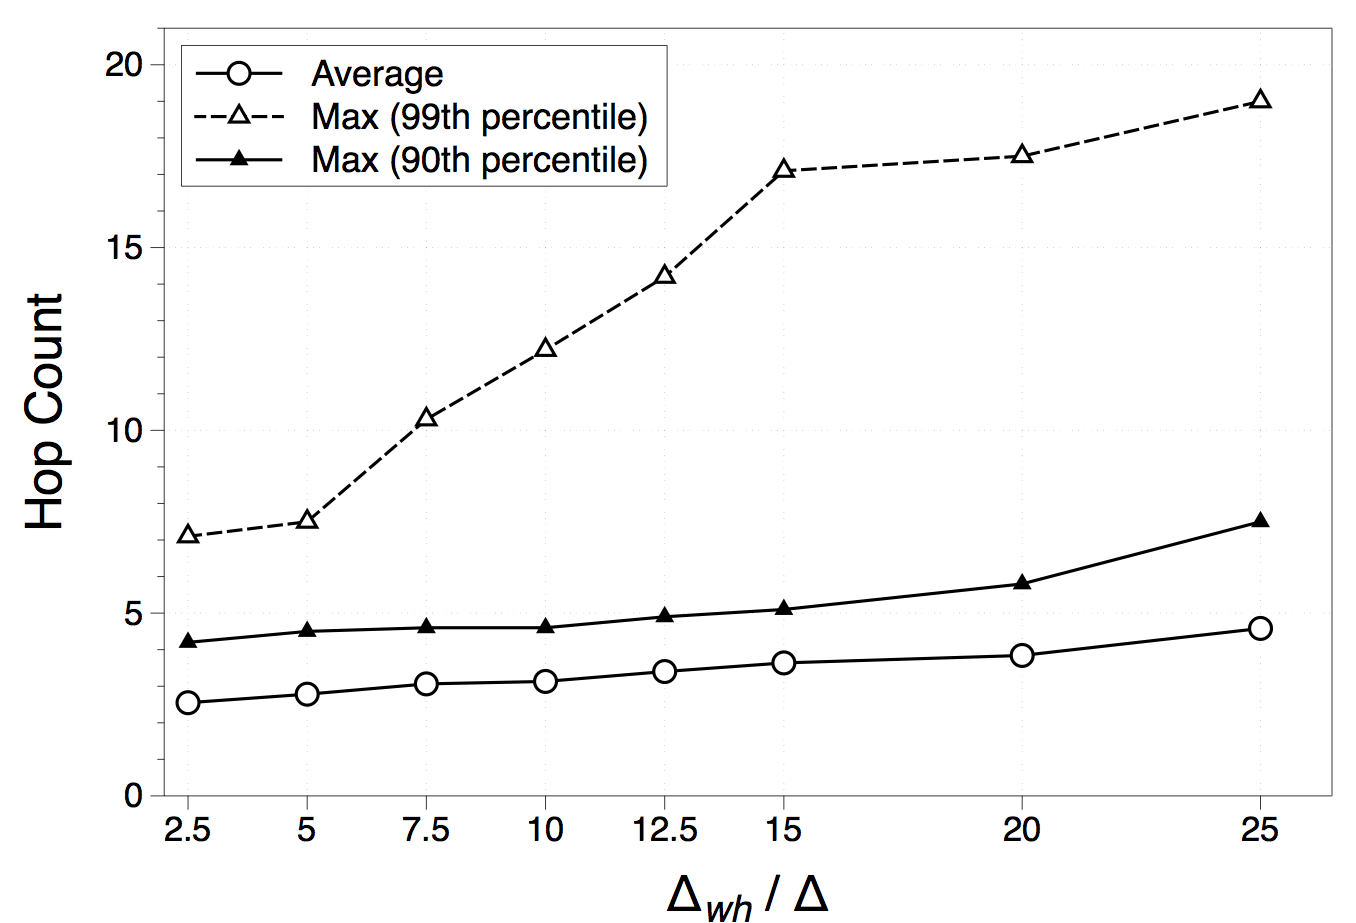
\includegraphics[keepaspectratio=true, width=\textwidth]{images/paper_average_hop_count}\caption{Test of average hop count reported in the paper}
  \label{fig:paper_average_hop_count}
\end{figure}

\section{Randomness}
\label{sec:eval_randomness}
As in \cite{wormhole}, we now want to evaluate the global randomness properties of our system by measuring properties of the WPSS overlay topology, so the upper overlay. This overlay is built connecting to all the samples stored at nodes. In this set of experiments, we measure the in-degree distribution of the WPSS overlay network, its convergence time for different view sizes, and finally its clustering coefficient for different view sizes. In Fig.~\ref{fig:converged_indegree} we can see the converged in-degree distribution. Obviously this result shows that the 95\% of the nodes have an in-degree included between 43 and 55, however there are some nodes that still have a quite large in-degree: these peers are the public nodes, which are initially present in a lot of views, so they have a large in-degree. This result is a little bit different from the original paper, in which they show that all the nodes have an in-degree included between 43 and 60. This is probably due to the environment, because they tried this set of tests in their deployed system, with 12000 nodes and for a long time. 
\begin{figure}[ht]
  \centering
  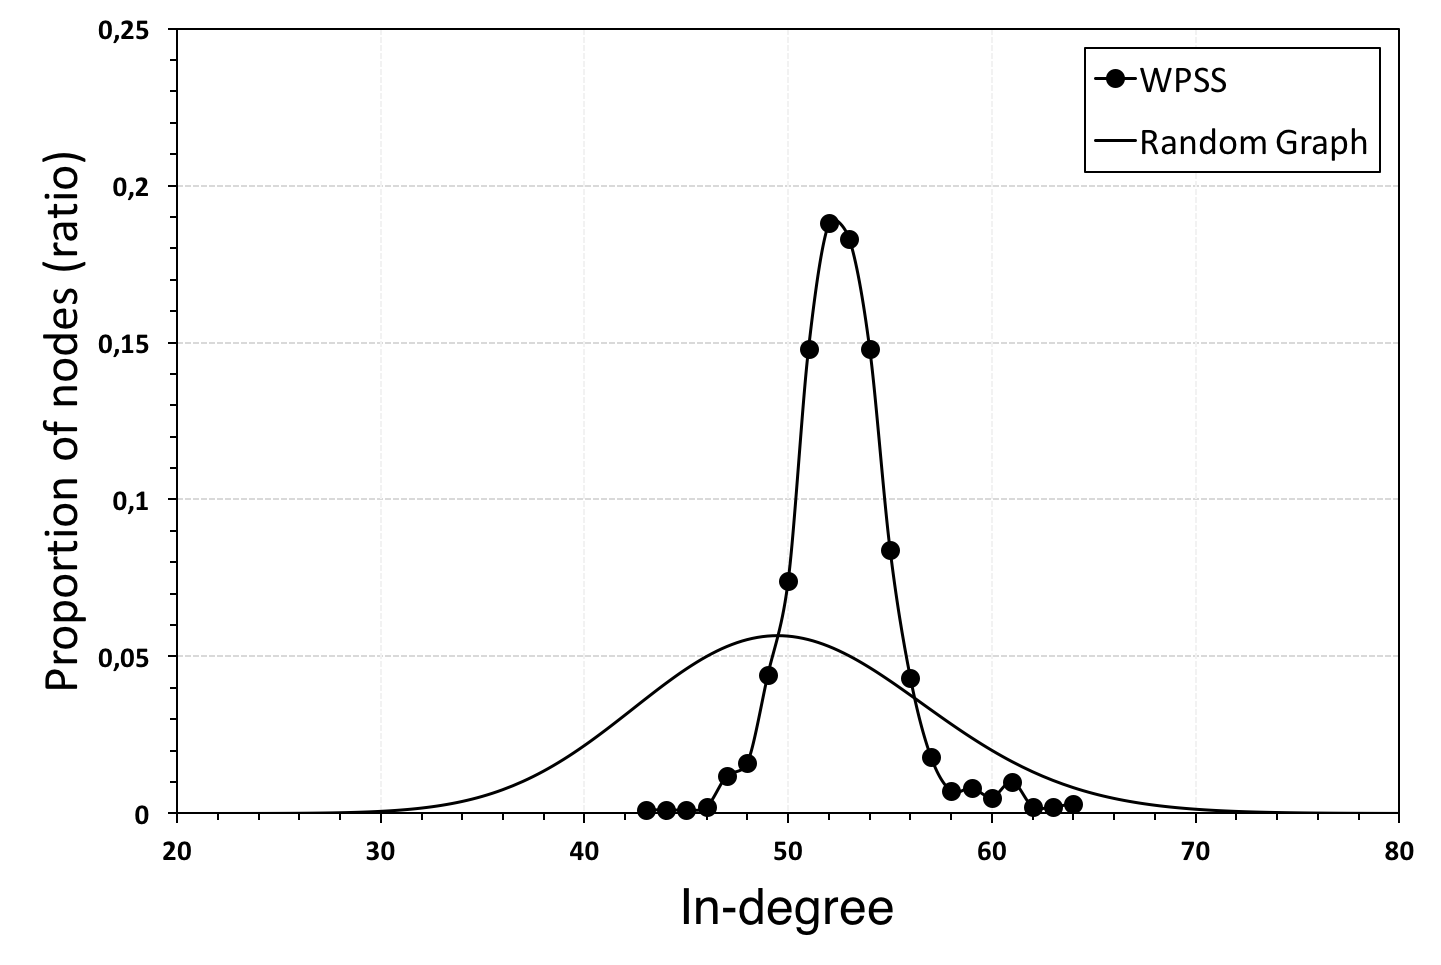
\includegraphics[keepaspectratio=true, width=\textwidth]{images/converged_indegree}\caption{Converged in-degree distribution}
  \label{fig:converged_indegree}
\end{figure}

One interesting fact, that confirms that the problem is not the implementation, is shown in Fig.~\ref{fig:indegree_evolution}: as we can see the in-degree converges to 50 after 4 minutes, and the standard deviation after 8 minutes, which are exactly the same results of the original paper, shown in Fig.~\ref{fig:paper_indegree_evolution}. If we look at this result, we are right to believe that running our implementation for a longer time and with an higher number of nodes could change the result obtained in the converged in-degree graph.

\begin{figure}[ht]
  \centering
  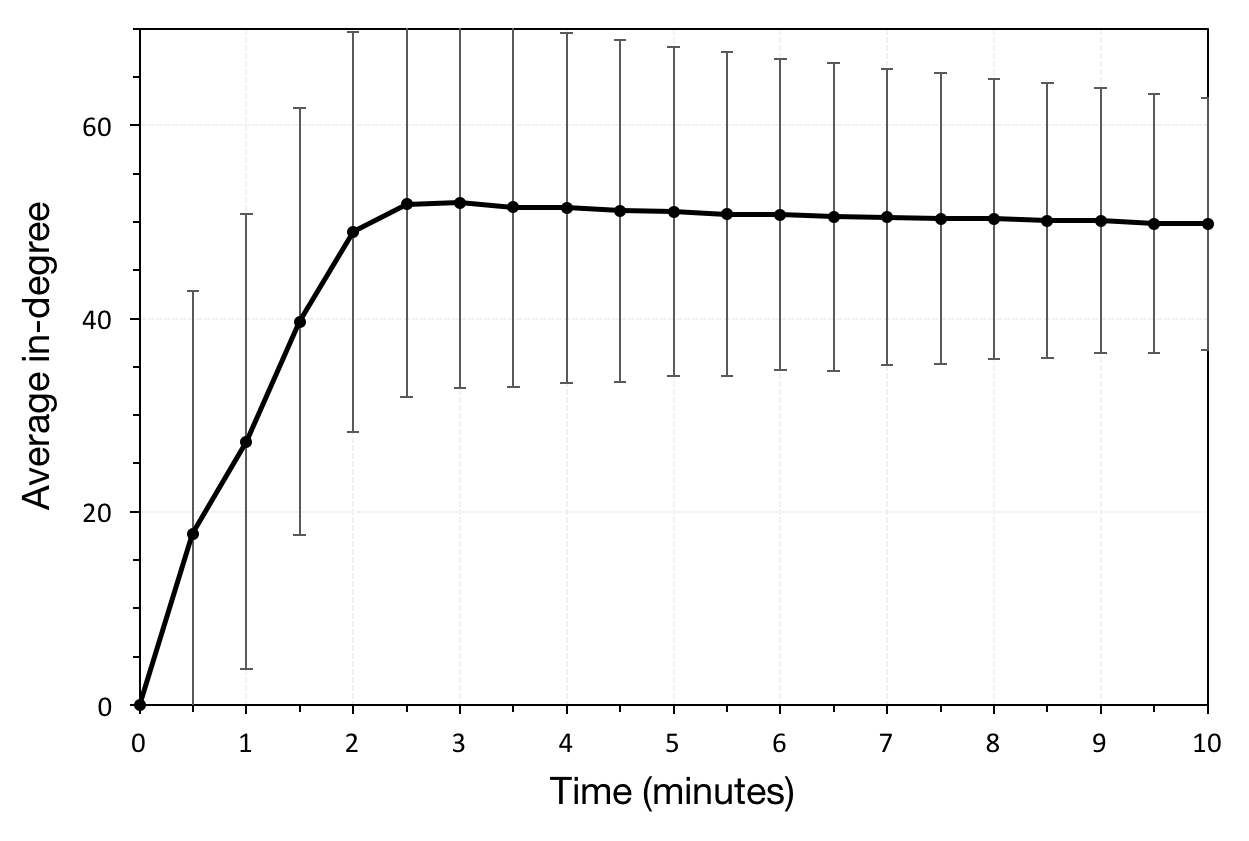
\includegraphics[keepaspectratio=true, width=\textwidth]{images/indegree_evolution}\caption{In-degree evolution over time with error bars}
  \label{fig:indegree_evolution}
\end{figure}

\begin{figure}[ht]
  \centering
  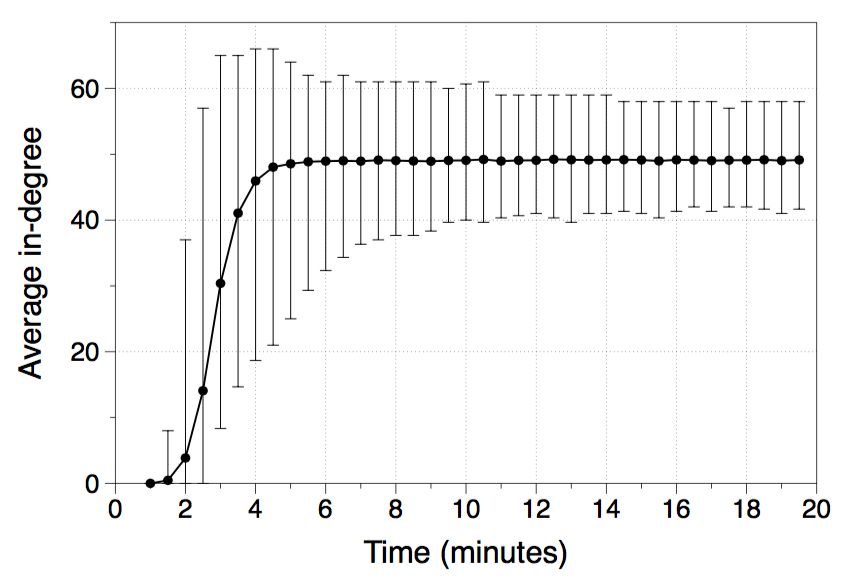
\includegraphics[keepaspectratio=true, width=\textwidth]{images/paper_indegree_evolution}\caption{Test of in-degree evolution reported in the paper}
  \label{fig:paper_indegree_evolution}
\end{figure}

\begin{figure}[ht]
  \centering
  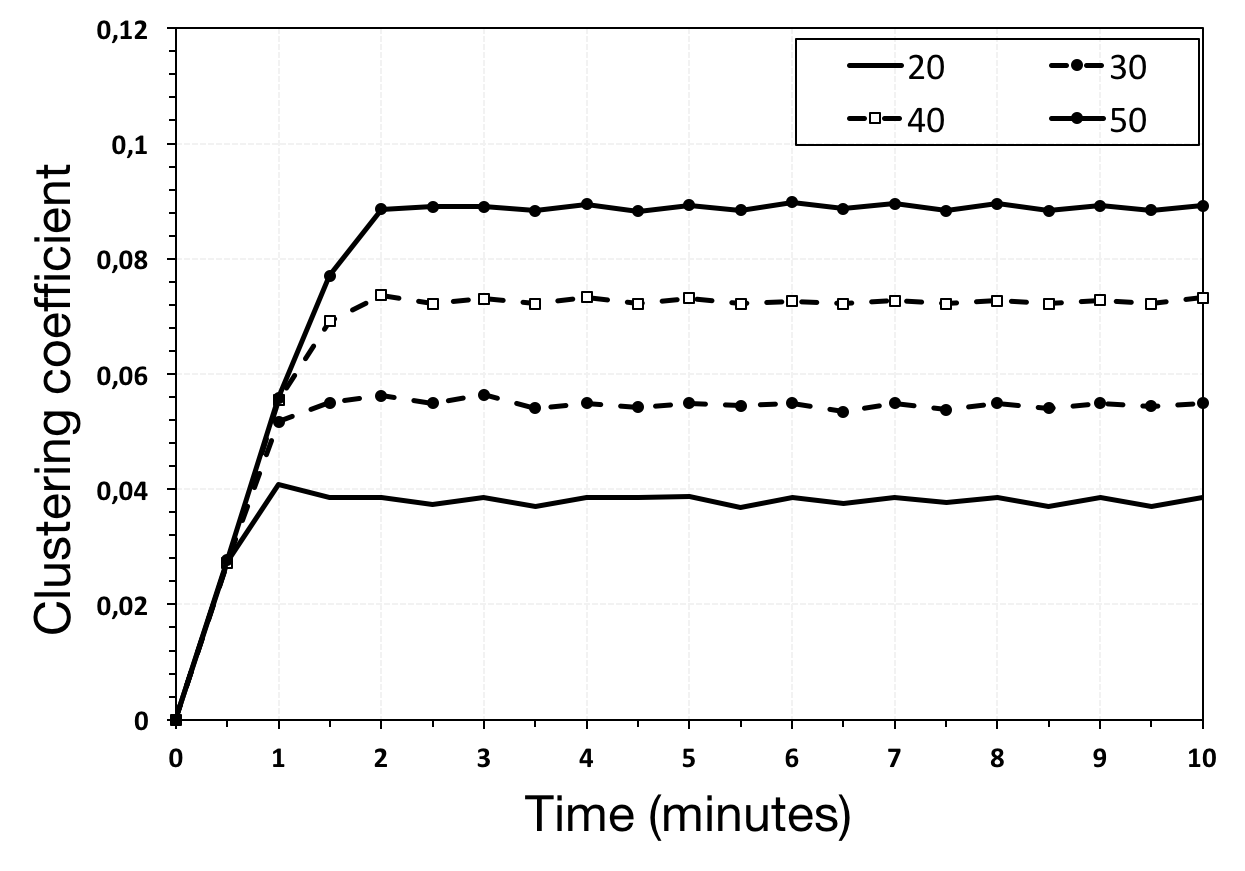
\includegraphics[keepaspectratio=true, width=\textwidth]{images/clustering_coefficient_evolution}\caption{Clustering coefficient evolution for different view sizes}
  \label{fig:clustering_coefficient_evolution}
\end{figure}

Fig.~\ref{fig:clustering_coefficient_evolution} shows the clustering coefficient evolution for different view size, as we can notice it grows with increasing the view size. In fact the higher the view, the higher the number of connections. This result is the same on the original paper. We can also notice that it converges roughly at the same rate as the in-degree.
The last test is shown in Fig.\ref{fig:converged_clustering_coefficient} and it indicates that the clustering coefficient is higher than the one of the random graph by a constant factor, which is due to the fact that WPSS does not guarantee independent samples at nodes that are close in the stable base overlay~\cite{wormhole}.

\begin{figure}[ht]
  \centering
  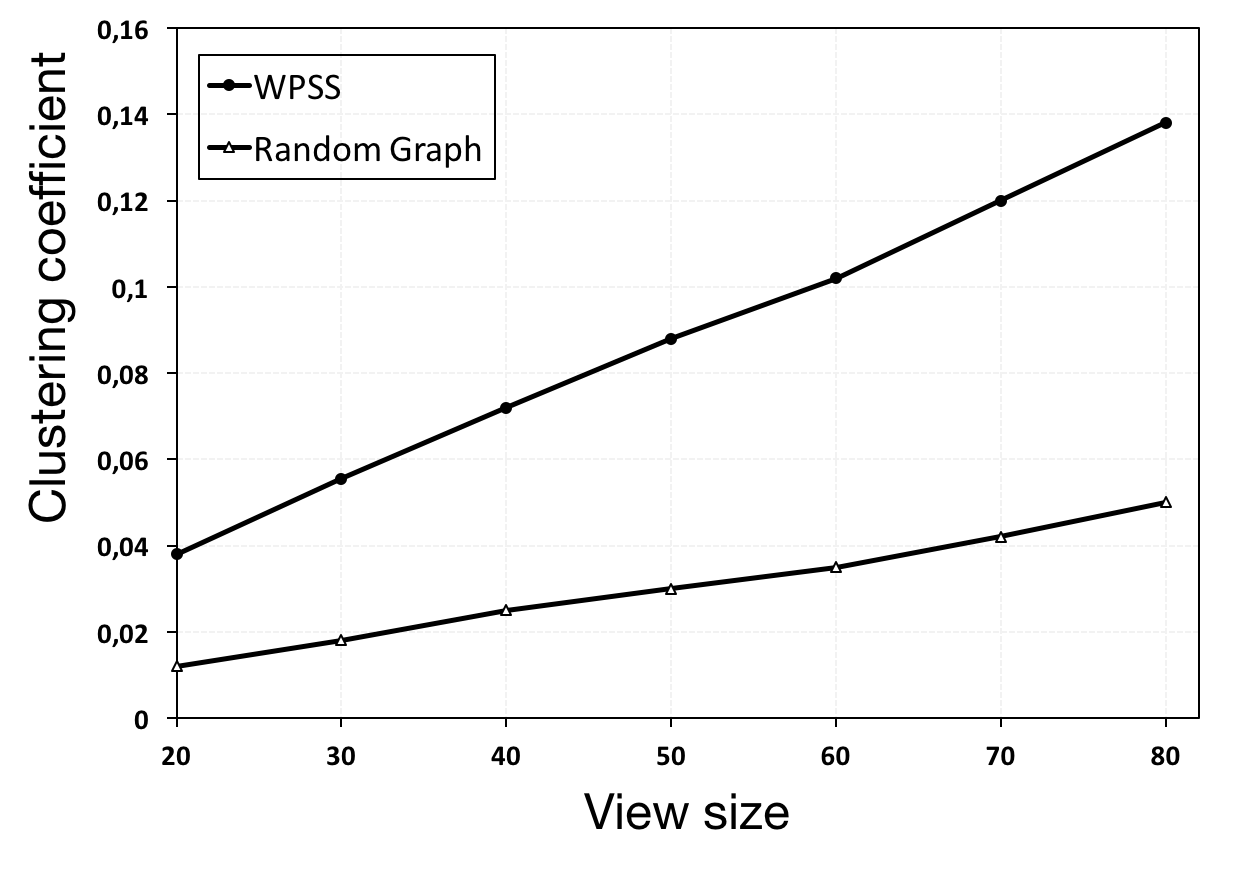
\includegraphics[keepaspectratio=true, width=\textwidth]{images/converged_clustering_coefficient}\caption{Converged clustering coefficient for in- creasing view sizes}
  \label{fig:converged_clustering_coefficient}
\end{figure}

\section{Inter-arrival Time of Advertisements}
\label{sec:interarrivaltime}
In these tests we want to measure the inter-arrival time of the advertisements, so the lapse of time between two consecutive accepted samples. This is an important factor, because the topology is a constraint: in fact the public nodes have a lot of peers connected to them, so they receive more advertisements than the private nodes that are connected only to few nodes. However, the \textit{acceptAd} method takes care of this: it ensures that all the nodes, in average, consume the advertisements at the same rate, namely one in each $\Delta$ period. In Fig.~\ref{fig:average_interarrivaltime} we can observe that the average inter-arrival time of the samples converges to the wormhole period $\Delta$ after about 2 minutes. Except in this time lapse, all the nodes in average consumes one advertisement every $\Delta$, which is exactly the result we were searching. Furthermore, this result is identical to the one shown in the original paper.

Now we want to verify if the \textit{acceptAd} method correctly balances samples across public and private nodes. To do that, we measured the difference inter-arrival time between them. As shown in Fig.~\ref{fig:interarrivaltime_difference} this difference is very low, about $500 ms$ in the worst case in which $\Delta = 6 s$. With $\Delta$ equals to $1s$ or $3s$ the difference is lower, about $100ms$ and $200ms$, so we can confirm that the \textit{acceptAd} method successfully balances the samples between all the nodes, as well as in the original paper.

\begin{figure}[ht]
  \centering
  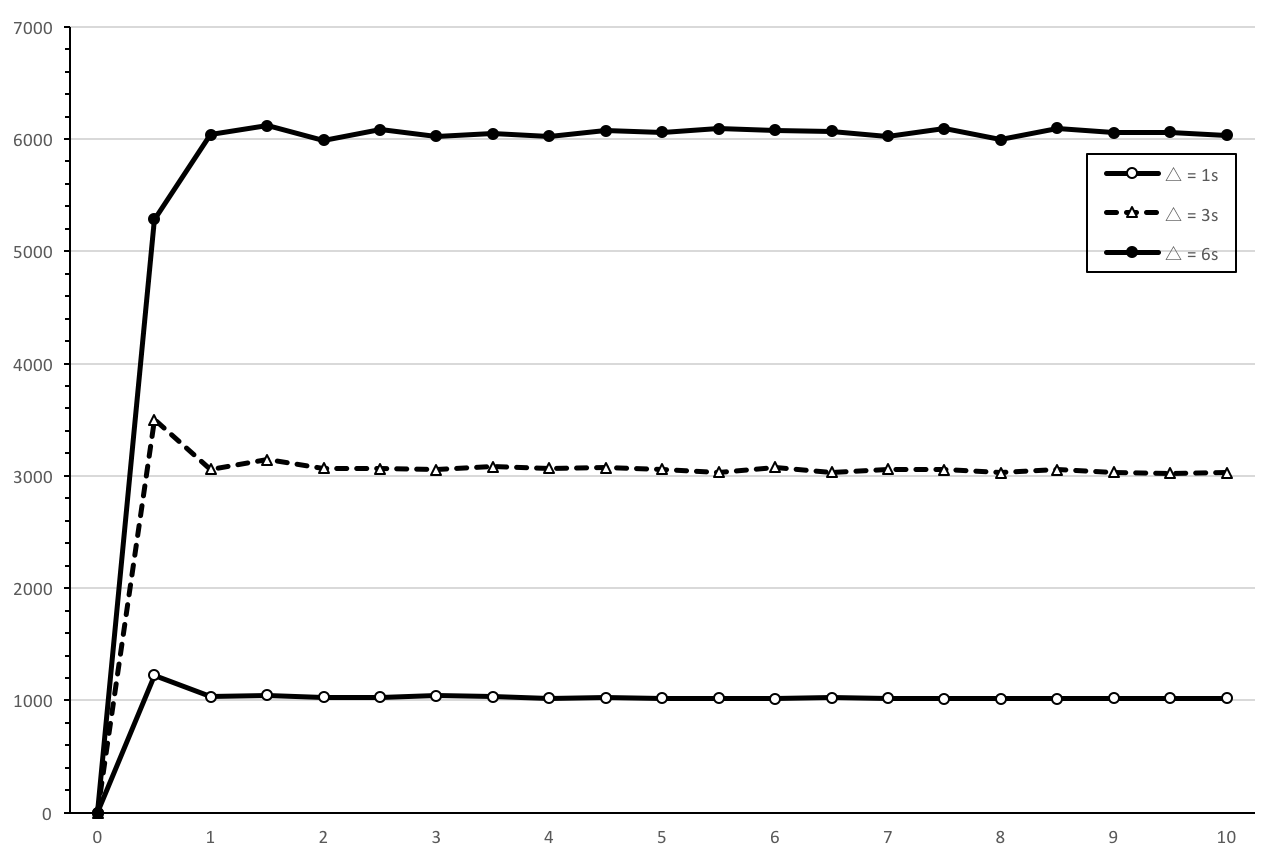
\includegraphics[keepaspectratio=true, width=\textwidth]{images/average_interarrivaltime}\caption{Average inter-arrival time for samples (terminating advertisements) at all peers}
  \label{fig:average_interarrivaltime}
\end{figure}

\begin{figure}[ht]
  \centering
  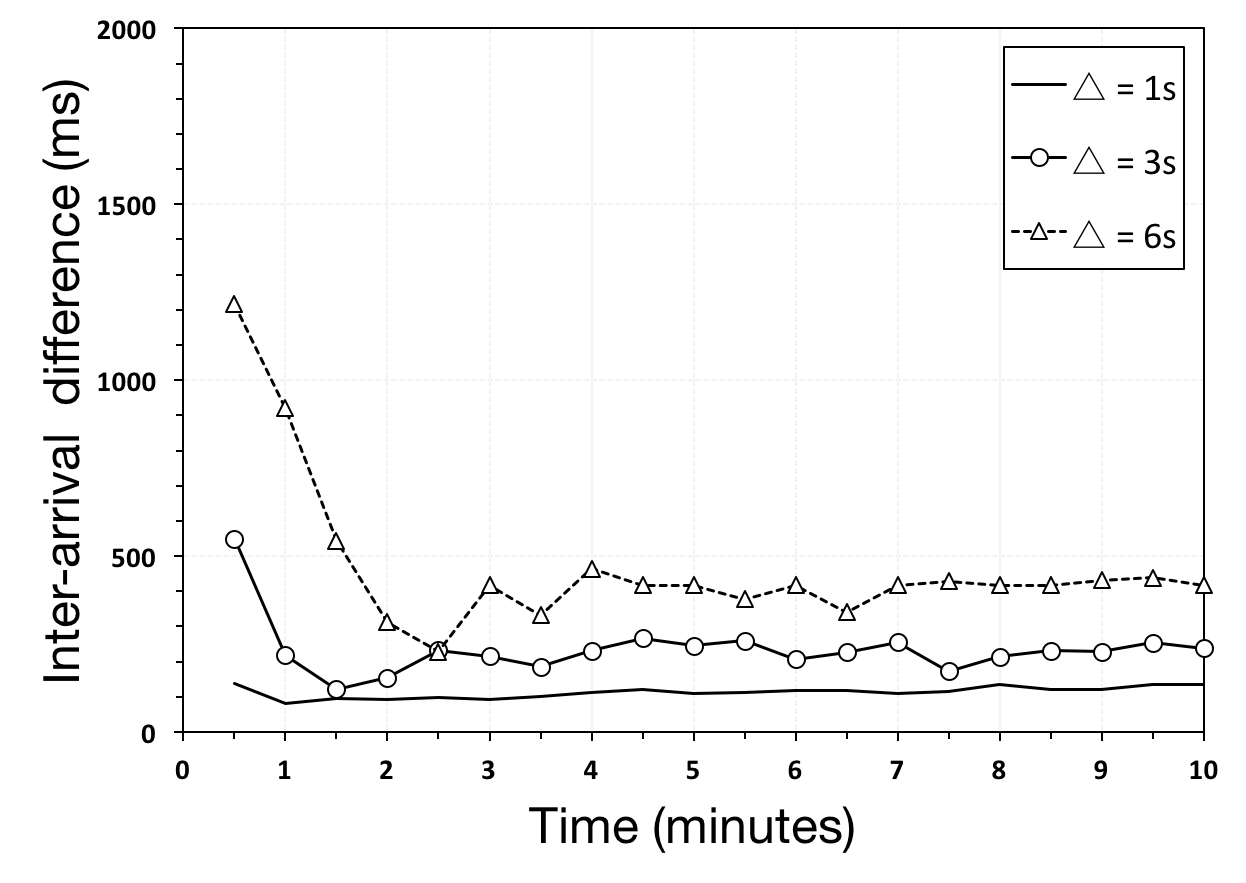
\includegraphics[keepaspectratio=true, width=\textwidth]{images/interarrivaltime_difference}\caption{Difference in inter-arrival time between public and private peers}
  \label{fig:interarrivaltime_difference}
\end{figure}

\section{Robustness to Different Churn Patterns}
\label{sec:robustness}
In this set of experiments we want to test the robustness of our implementation under different levels of churn. We measure the average hop count, as well as the clustering coefficient and the in-degree. In the first three experiments we recreate a flash crowd scenario, in which some nodes join at the beginning and the remaining join at a later point in time. For instance, recalling that $N = 1000$, for a flash crowd scenario of 70\% of the node, 300 nodes join at time $0s$ and 700 nodes join at minute $6.5$. So after this time, the number of nodes stays constant at 1000. In Fig.\ref{fig:average_hop_count_flash_crowd} we can see that the average hop count increases with decreasing the number of nodes that join the system at time 0, in fact an advertisement will have to traverse more nodes in order to reach a peer that does not already have that sample. However at time $6.5$, when all the remaining nodes join the system, the average hop count not only it stabilizes quickly, but it converges to the same value in all the experiments. In Fig.~\ref{fig:paper_average_hop_count_flash_crowd} is shown their result and as we can see they are identical, they also stabilize at the same rate. The next test measures the clustering coefficient in a flash crowd scenario, the expected behavior is similar to the average hop count. As shown in Fig.\ref{fig:average_clustering_coefficient}, this is the case. In fact the clustering coefficient stabilizes quickly and to the same rate when all the nodes join the network. Finally, Fig.\ref{fig:average_indegree} shows the average in-degree of the nodes. As we can see after two minutes in all the experiments the nodes have in average the same in-degree, then it drops significantly at time $6.5$, this is in fact expected since a majority of the nodes join the network with in-degree equals to 0. However, it recovers quickly (about $1.30$ minutes later) and it converges to 50 in all the experiments.

In the next set of experiments we measure the robustness of our implementation in case of catastrophic failures, that is, when a large number of peers leaves the system at a single instant in time. All the nodes join the system at time $0$, we wait for the overlay to stabilize and then we fail a fixed percentage of nodes at time $5$ minutes. We expect that the algorithm recovers quickly and also that all the nodes remain connected, even in the worst case scenario where 80\% of the peers leave the system. In Fig.\ref{fig:average_hop_count_failures} we can notice that all the experiments has the same average hop count until time $5$ minutes, then it increases with increasing of failures. This is expected given the large number of broken links to detect and repair for both the base and wormhole overlays. Notice that the network remains connected even when 80\% of the nodes fail. Fig.~\ref{fig:average_clustering_coefficient_failures} shows the evolution of the clustering coefficient: it increases with increasing of failures, since there are less nodes in the network and they are much more connected between each other. One important experiment in case of massive failures is to measure the average number of dead links in the views of the peers. What we want to obtain is a system which detect and replace the broken links as fast as possible. Fig.~\ref{fig:average_dead_links} shows the result: at time $5$ the number of dead links increases (obviously the higher the failures, the higher the number of dead links), however after just one minute all the broken links are successfully deleted from the views (even in the worst case where 80\% of the nodes fail), and the average number returns equals to zero. This result is even better of the one shown in the original paper, because the time employed by them to replace the links is two minutes, we do it in half time. This is probably due the fact that we use a tracker, which has high availability and it responds to all the nodes immediately, while they use the random walks, so they need more time to find a node and establish a new network connection.

\begin{figure}[ht]
  \centering
  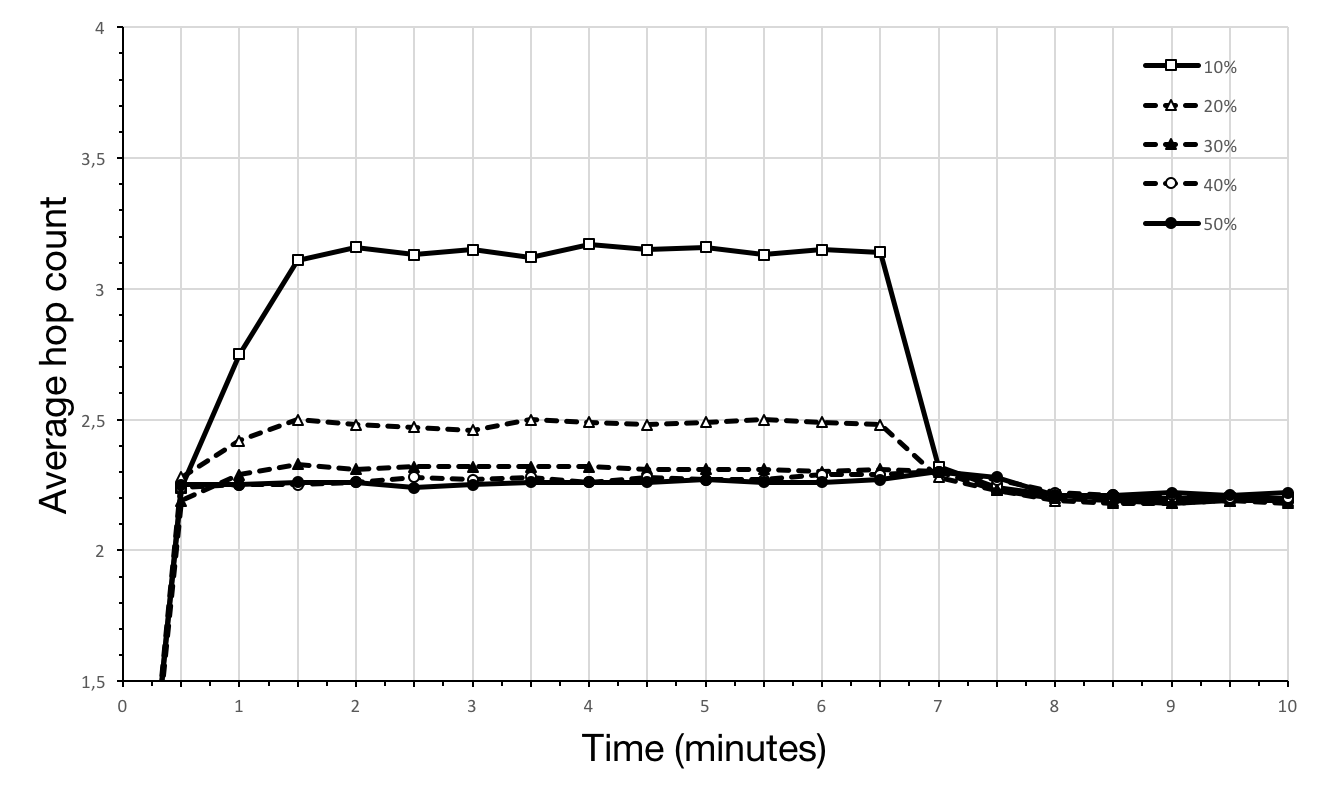
\includegraphics[keepaspectratio=true, width=\textwidth]{images/average_hop_count_flash_crowd}\caption{Average hop count}
  \label{fig:average_hop_count_flash_crowd}
\end{figure}

\begin{figure}[ht]
  \centering
  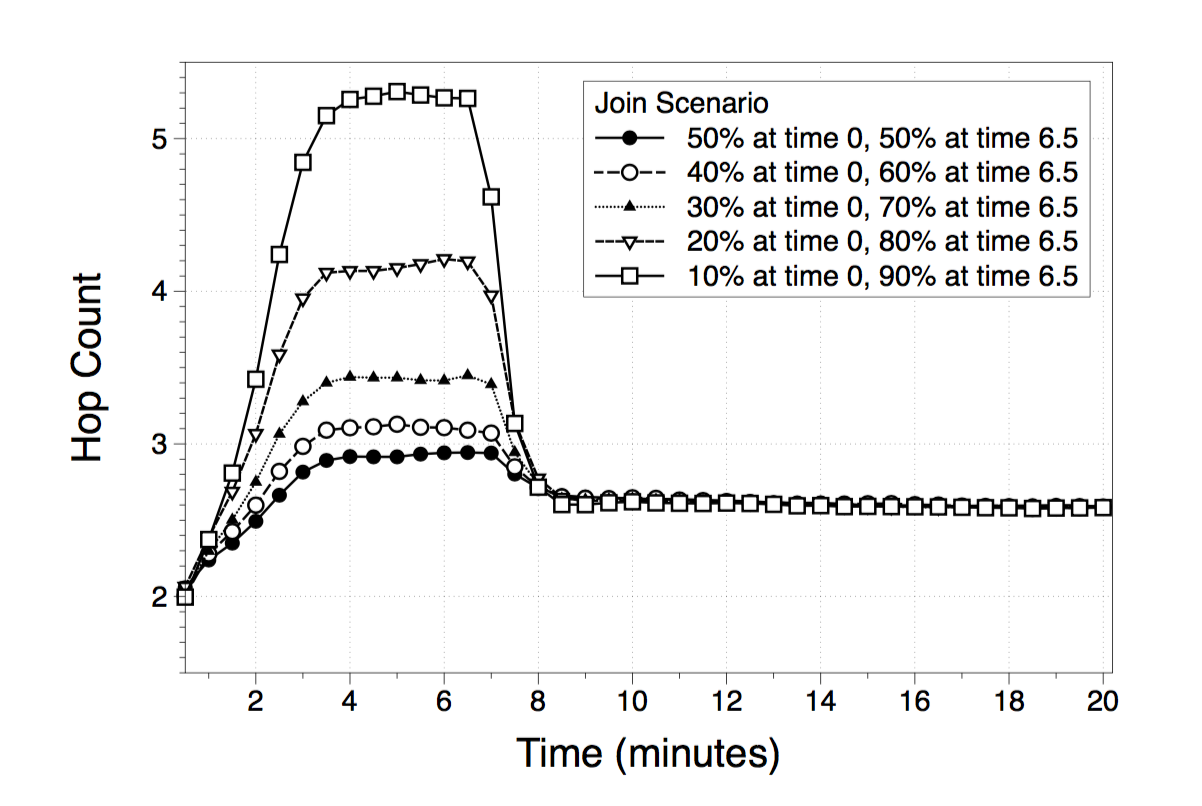
\includegraphics[keepaspectratio=true, width=\textwidth]{images/paper_average_hop_count_flash_crowd}\caption{Test of the average hop count in a flash crowd scenario reported in the paper}
  \label{fig:paper_average_hop_count_flash_crowd}
\end{figure}

\begin{figure}[ht]
  \centering
  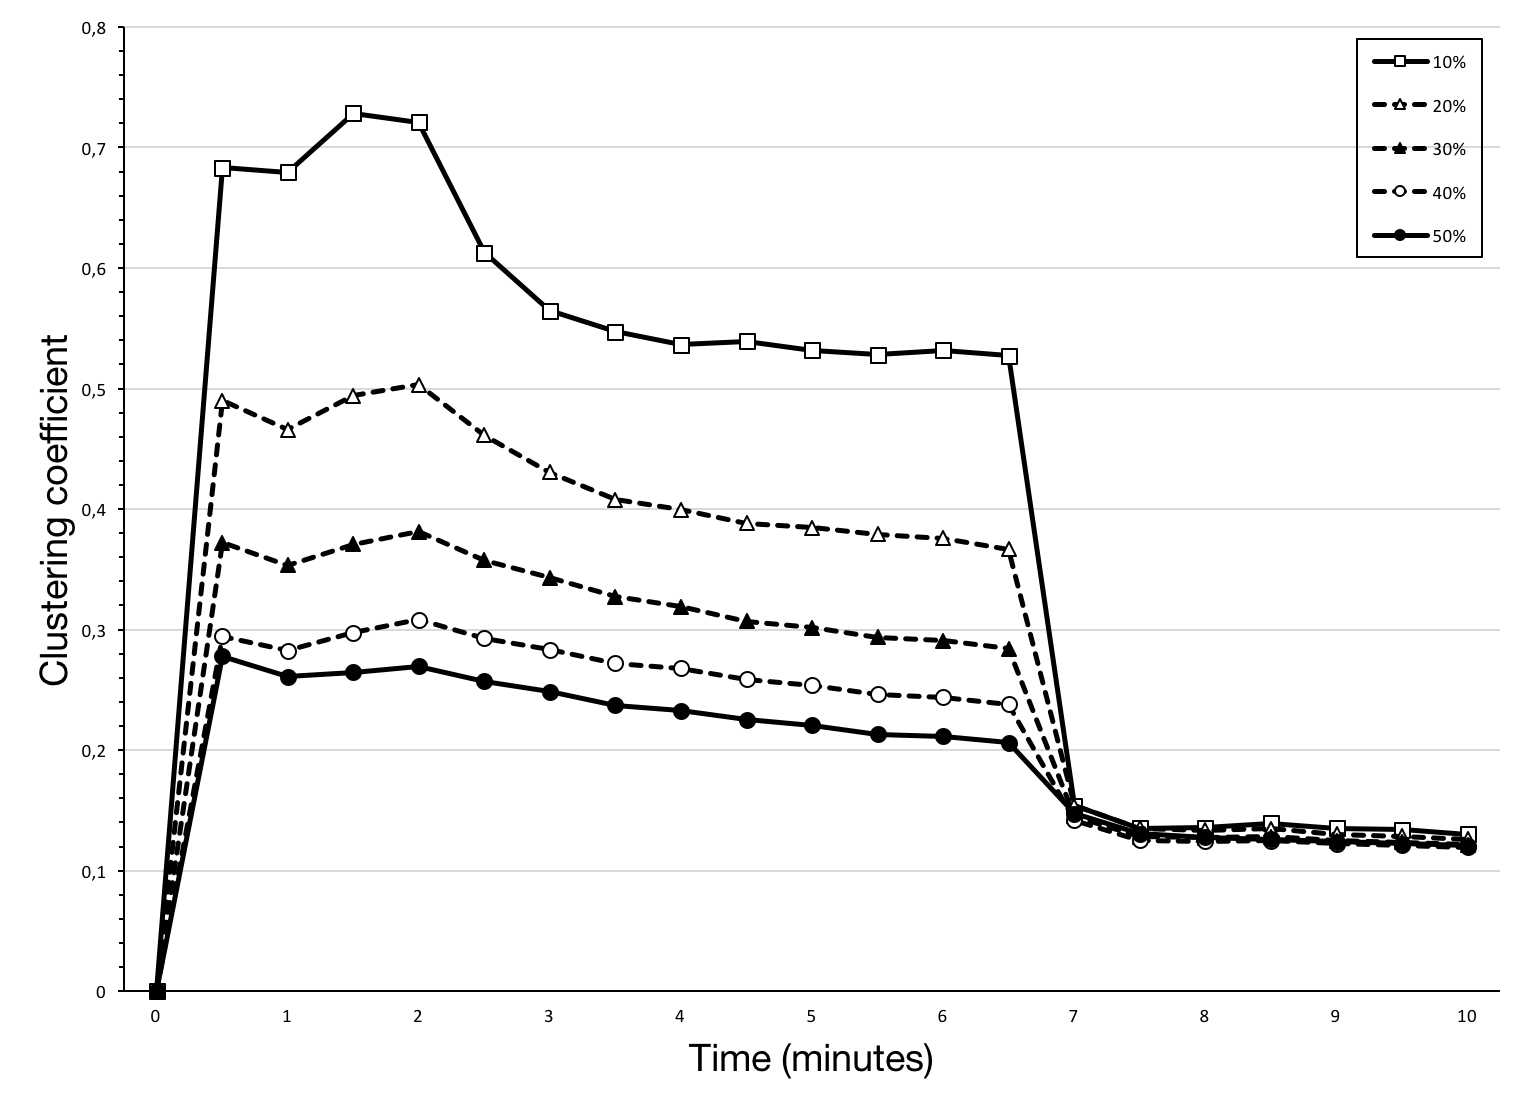
\includegraphics[keepaspectratio=true, width=\textwidth]{images/average_clustering_coefficient}\caption{Average clustering coefficient}
  \label{fig:average_clustering_coefficient}
\end{figure}

\begin{figure}[ht]
  \centering
  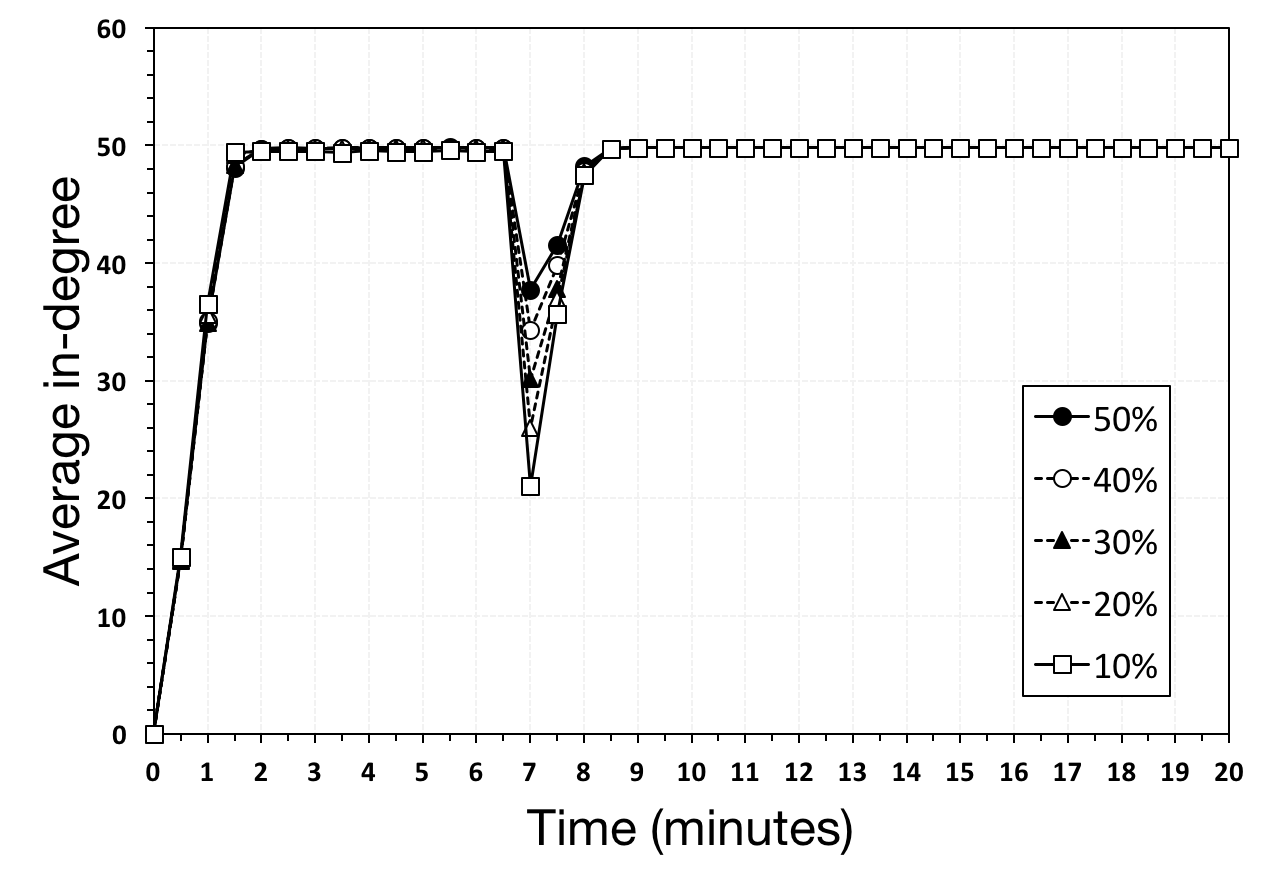
\includegraphics[keepaspectratio=true, width=\textwidth]{images/average_indegree}\caption{Average in-degree}
  \label{fig:average_indegree}
\end{figure}

\begin{figure}[ht]
  \centering
  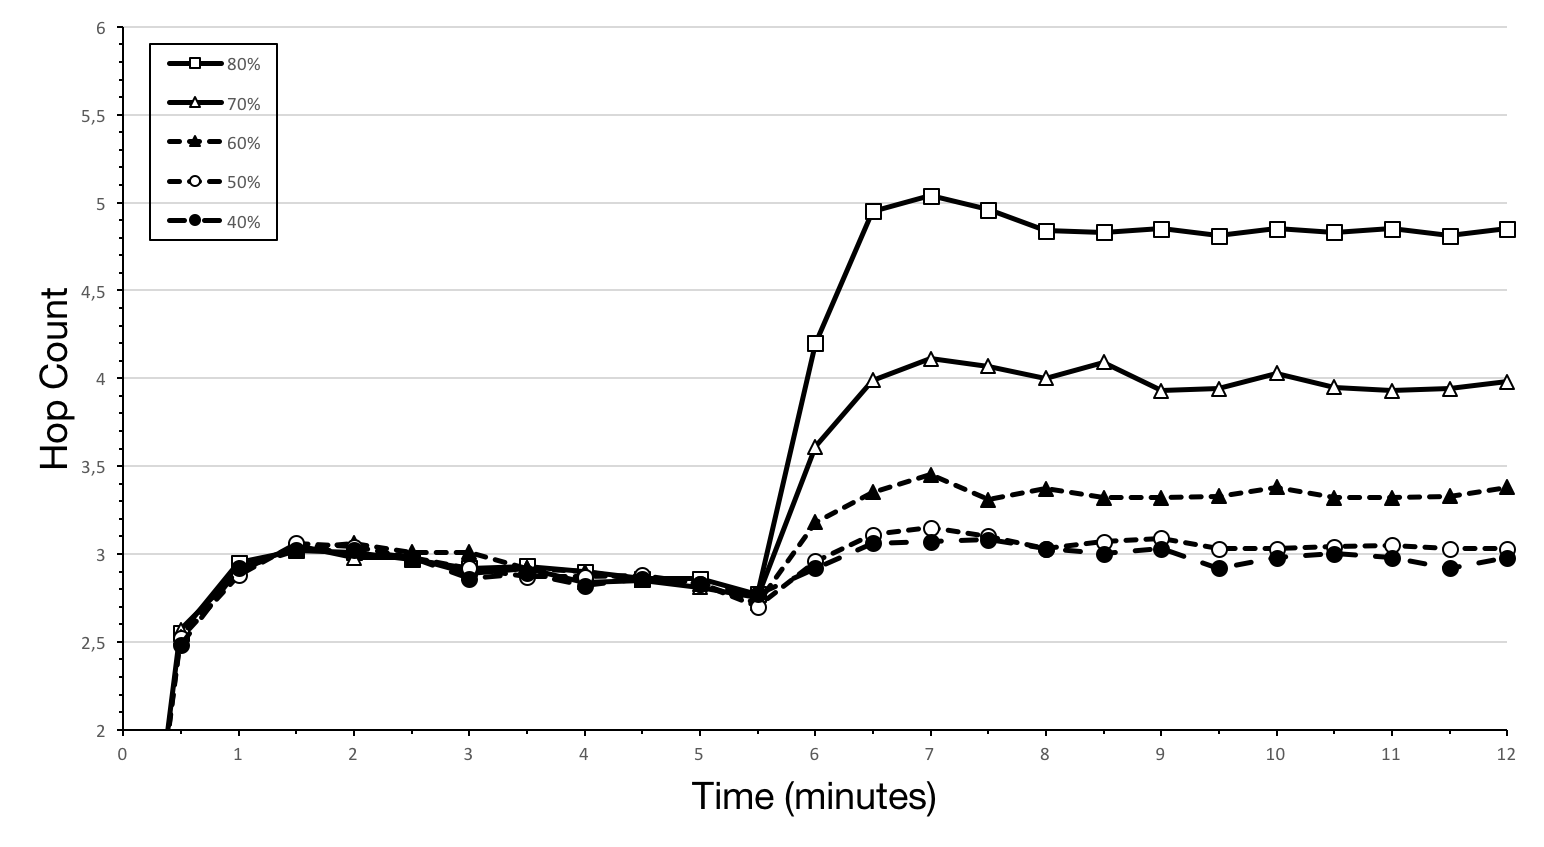
\includegraphics[keepaspectratio=true, width=\textwidth]{images/average_hop_count_failures}\caption{Average hop count}
  \label{fig:average_hop_count_failures}
\end{figure}

\begin{figure}[ht]
  \centering
  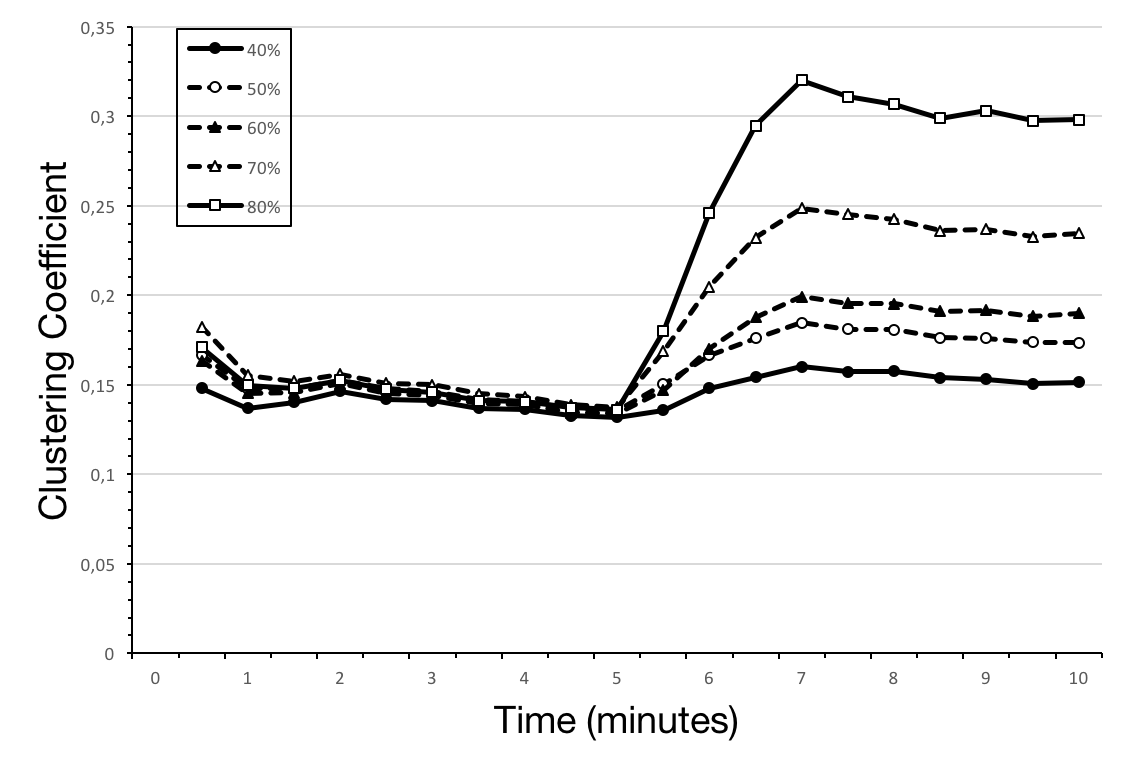
\includegraphics[keepaspectratio=true, width=\textwidth]{images/average_clustering_coefficient_failures}\caption{Average clustering coefficient}
  \label{fig:average_clustering_coefficient_failures}
\end{figure}

\begin{figure}[ht]
  \centering
  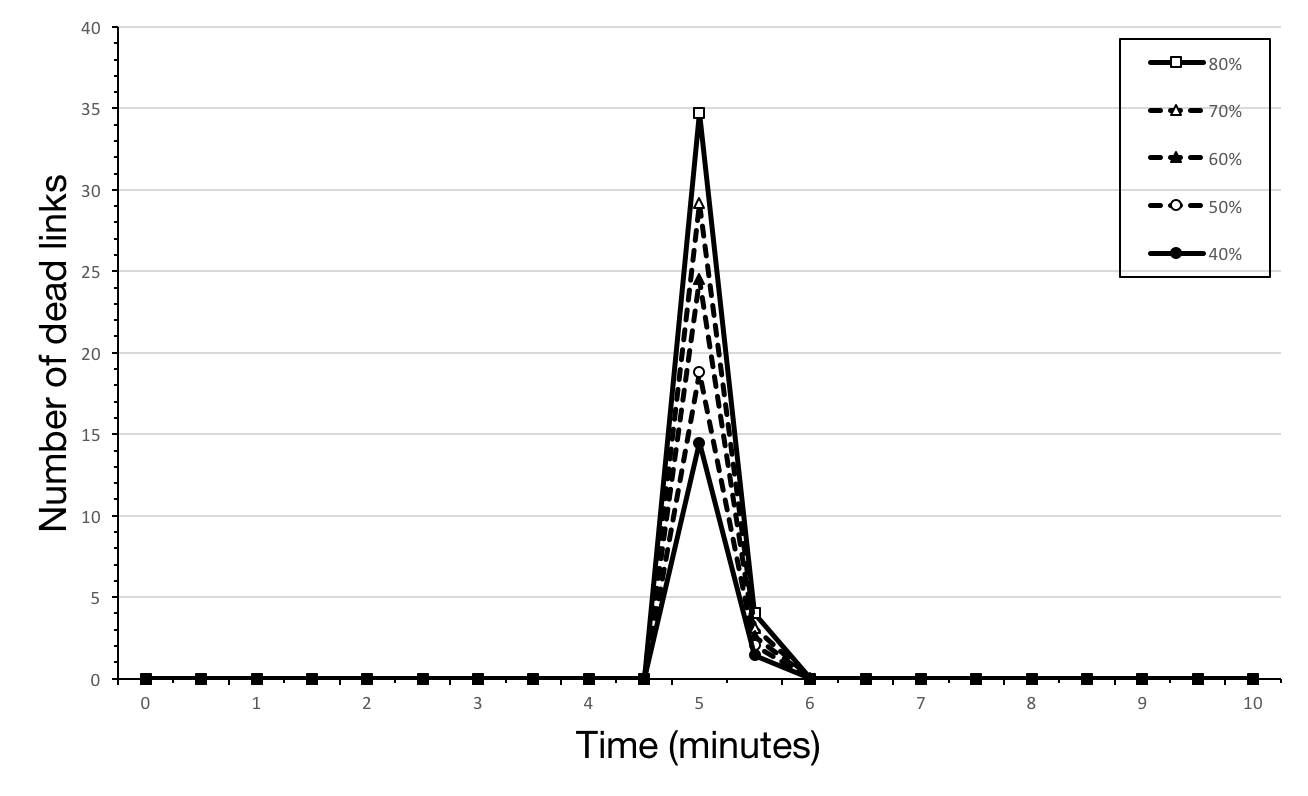
\includegraphics[keepaspectratio=true, width=\textwidth]{images/average_dead_links}\caption{Average number of dead links in view}
  \label{fig:average_dead_links}
\end{figure}
